\chapter{Gate defined triangular cavities}

In this chapter, we simulate a gate defined triangular cavity and describe its operation as a switch that couples different MBS pairs.
The device is built using a stack with three layers of materials: 2DEG, dielectric and metallic gates.
The electrostatic potential inside the 2DEG is found as the solution to Eq. \eqref{eq: laplace} using the finite element solver from Ref. .

Two devices are simulated in order to study the angular dependence previously found.
First, we discuss the tuning of each device such the potential resembles the triangular cavity and the nanowires are strongly coupled.
Then, the MBS coupling is calculated and compared to the purely geometric case.

\section{Gates configuration}

\begin{figure}[h!]
\centering
  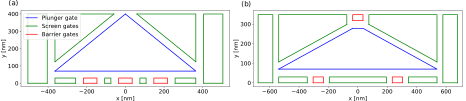
\includegraphics[width=\linewidth]{figures/gate_configurations.pdf}
  \caption{Gate configuration of the two triangular cavities considered. The area is set $A=1200$ $[a^2]$. (a) Triangular cavity with angle $\theta = 0.234 \pi$ with all nanowires at the lower side. (b) Triangular cavity with angle $\theta = 0.125\pi$ with central nanowire at the top side. Spacing between gates is set to $40$ nm. Barrier gates have length $30$ nm and width $70$ nm. Nanowires (not shown) are attached at the ends of the barrier gates. The vertical configuration includes a 2DEG of thickness $40$ nm. Then follows an insulating layer of thickness $40$ nm, and finally the metallic gates of thickness $60$ nm.}
  \label{fig:gates}
\end{figure}

A trijunction is a complex Majorana device that can be implemented on a 2DEG by selectively depositing electrostatic gates.
It contains two main regions: three nanowires and a semiconducting cavity.
We focus on the design of a gate defined triangular cavity.
We do not consider the electrostatic modeling of the nanowires since one can assume that the electric field in the nanowires is screened by the superconductor.

The gates are placed in a single layer above the 2DEG with a dielectric layer in between.
Different layer configurations were explored, and a single layer was found to be the best in terms of shape-resolution and voltage range.
The thickness of each layer determines how much the electric field penetrates into the 2DEG.
We consider typical parameters from experiments as described in the inset of Fig. \ref{fig:gates}.

In contrast to the geometrical model discussed in the previous chapter, the triijunction is defined in a smooth potential landscape.
The global potential is affected by all involved gates.
There are three kinds of gates:
\begin{enumerate}
\item Plunger gate: Defines and controls the potential inside the triangular cavity region.
\item Screen gates: There are two kinds of screen gates: First, the triangular screen gates deplete the 2DEG around the plunger gate, which contributes to the overall triangular shape. Second, the screen barrier gates between the tunnel gates that keep each nanowire channel separated from the others.
\item Barrier gates: Modulate the coupling between each nanowire and the cavity. They allow to tune the system in the insulating, tunnelling, and strong coupling regimes.
\end{enumerate}

In general terms, to operate the device optimally we require the minimum number of tunable gates while having enough flexibility to connect different MBS pairs.
There are two basic requirements that must be satisfied at all times:
\begin{enumerate}
\item Electron density inside the cavity is placed under the plunger gate.
\item Selectively couple different pairs of MBS via the cavity by tuning the barrier gates. The last MBS remains decoupled.
\end{enumerate}
These two requirements require us to calibrate the tunnel and the screen gates separately.
At the same time, one has to vary the minimum number of gate voltages while maximising the coupling.
In the remaining of this section, we discuss how these conditions can be satisfied in both devices.

\section{Device 1}

\begin{figure}
\centering
  \includegraphics[width=\linewidth]{figures/device_1_potential.pdf}
  \caption{Equipotential lines inside the device for representative parameters of the (a) left and right MBS pair and (b) left and center MBS pair. Colorbar indicates value of equipotential lines. (c) Cut of the potential along the tunnel barriers, i.e. dashed black lines in (a) and (b), taken for a range of plunger gate voltages. Colorbar in (c) indicates the plunger gate voltage.}
  \label{fig:device_1_barriers}
\end{figure}

In this section we describe the operation of the gate configuration shown in Fig. \ref{fig:gates} (a).
Interestingly, this device allows us to explore geometric deformation beyond the triangular cavity by tuning the triangular screen gates.
In Fig.  \ref{fig:device_1_barriers} (a) - (b) one can observe the potential inside the 2DEG for the coupling of each pair.
One can observe that the triangular walls are well defined in the potential, but inside the triangle the bottom of the potential has a different shape.

In Fig. \ref{fig:device_1_barriers} (c) one can observe that a double well is created when coupling a given pair of MBS.
For the left and right MBS pair (upper panel) the potentials remain well separated.
On the other hand, the central pairs are very close and the screen barrier can be lowered below the MBS potential, allowing for direct coupling.
To explore potential deformations it is required that the tunnel channels to the nanowires remain separated.

\subsection{Nanowire channels}

\begin{figure}
\centering
  \includegraphics[width=\linewidth]{figures/device_1_barriers.pdf}
  \caption{Coupling of (a) left and right MBS pair and (b) left and central MBS pair as a function of the corresponding barrier gates. Orange and blue lines indicate when the potential at the bottom of the barriers crosses $0$ V or the MBS potential, $\mu_0$. Plunger gate is tuned around the first resonance. Gate voltages used correspond to those described in Table \ref{table:gate_voltages_1}.}
  \label{fig:device_1_barriers}
\end{figure}

Operating the left and right tunnel barriers is straightforward since they are far from each other.
Consequently, there is no interdependence between them as can be observed in Fig. \ref{fig:device_1_barriers} (a).
On the other hand, the operation of the central pairs is not symmetric given the mutual influence of successive barrier gates.
In Fig. \ref{fig:device_1_barriers} (b) one can observe that the slope of the potential crossings suggests a mutual interaction between successive barrier gates.

The system can be tuned in the insulating, tunnelling, and strong coupling regimes by manipulating the barrier gates.
The blue and orange lines in Fig. \ref{fig:device_1_barriers} indicate the value of the potential at the bottom of the barrier gates with respect to $\mu_0$ and $0$, respectively.
The insulating regime corresponds to the region beyond the blue lines.
The tunnelling regime starts at the blue line, when the barrier potential crosses $\mu_0$.
In this regime, the coupling is mediated by direct overlap of the MBS wavefunctions.
Therefore, one observes a difference in the tunnelling regime of panels (a) and (b) since in the later the MBS are closer.
The orange lines indicate the start of the strong coupling regime.

As the barriers are lowered, there are two new effects:
On one hand, new crossings caused by resonant cavity levels appear.
On the other hand, for very large barrier gates, the MBS couple directly since the screen barrier is lower than $\mu_0$.
The former effect can be seen clearly in panel (a) as the two crossings in the strong coupling regime.
The later can be seen in the lower right part of panel (b) where the coupling increases due to direct coupling.
Keeping the barrier potential as small as possible within strong coupling decreases the influence of these effects.

\subsection{Background potential}

\begin{figure}
\centering
  \includegraphics[width=\linewidth]{figures/device_1_screens.pdf}
  \caption{Coupling of (a) left and right MBS pair and (b) left and central MBS pair as a function of the triangular screen gates. Three regimes of the electron density localisation are separated by the orange and blue lines. Plunger gate is tuned around the first resonance. Gate voltages used correspond to those described in Table \ref{table:gate_voltages_1}.}
  \label{fig:device_1_screens}
\end{figure}

The screen gates depleted the electronic density in the 2DEG such that is concentrated below the plunger gate.
In Fig. \ref{fig:device_1_screens} one can observe the MBS coupling as a function of the voltages of the two triangular screen gates for each pair.
First, one observes that below the orange lines, there some resonances with a small MBS coupling.
In this case, the density is not confined under the plunger gate, but electrons can move over the whole 2DEG.
By tuning the potential to more negative values, between the orange and blue lines, a region with large coupling develops, indicating that electrons are confined in the triangular region.
Further increasing the potential depletes the area under the plunger gate as can be seen beyond the blue line.
Observe that it takes higher voltages to reach this last regime in the case of panel (b).

In panel (a) one observes that the case of the left and right MBS pair is symmetric.
On the other hand, panel (b) shows an asymmetry for the left and central MBS pair.
Here the coupling increases by tuning one screen gate more negative than the other.
This is new regime for the coupling of the central MBS pairs that was not found in the purely geometric model.
One can understand this phenomena as an effectively size decrease for the cavity.
As the right screen gate increases, the left and central MBS overlap increases as can be observed.

\section{Device 2}

\begin{figure}
\centering
  \includegraphics[width=0.7\linewidth]{figures/device_2_potential.pdf}
  \caption{Equipotential lines inside the device for representative parameters of the (a) left and right MBS pair and (b) left and center MBS pair. Colorbar indicates value of equipotential lines. (c) Cut of the potential along the tunnel barriers, i.e. dashed black lines in (a) and (b), taken for a range of plunger gate voltages. Colorbar in (c) indicates the plunger gate voltage.}
  \label{fig:device_2_barriers}
\end{figure}

In this section we describe the operation of the gate configuration shown in Fig. \ref{fig:gates} (b).
In contrast to the previous device, here the interplay between barrier and screen gates is crucial to keep the nanowires connected to the cavity.
In Fig.  \ref{fig:device_2_barriers} (a) - (b) one can observe the potential inside the 2DEG for connecting each pair.
One observes that the barrier gates are well separated from each other, but the electron density below all of them depends in the surrounding screen gates as in the case of the top barrier in panel (b).

Since this device has a smaller angle, it resembles a quasi-one dimensional shape.
Observe that it is $800$ nm long and $150$ nm wide.
The wavefunctions will concentrate around the center of the cavity and not in the narrow edges.
Consequently, one can expect a larger coupling in the tunnelling regime, and resonant trapping for the left and right MBS coupling.
Furthermore, in panel (b) one can observe that the potential minima inside the cavity follows a narrow channel trajectory.
The far disconnected end of the triangular potential is higher, which implies a large deformation from the geometrical case.

\subsection{Nanowire channels}

\begin{figure}
\centering
  \includegraphics[width=\linewidth]{figures/device_2_barriers.pdf}
  \caption{Coupling of (a) left and right MBS pair and (b) left and central MBS pair as a function of the corresponding barrier gates. Plunger gate is tuned around the first resonance. Gate voltages used correspond to those described in Table \ref{table:gate_voltages_2}.}
  \label{fig:device_2_barriers}
\end{figure}

There are two differences with respect to the previous device:
First, since all barrier gates remain well separated from each other, there is no interdependence of barrier gates for any pair as one can observe in Fig. \ref{fig:device_2_barriers}.
Second, in the tunnelling regime, there is a significant coupling.
This is a consequence of how the gate geometry influences the spatial distribution of the wavefunctions.
In this device, the wavefunction concentration in the middle of the cavity is higher than in the previous device.

In the strong coupling regime there is a large difference between the coupling of the different pairs.
One can observe that panel (a) is similar to the previous device, which suggests that the triangular geometry effects are present in both devices.
On the other hand, panel (b) shows a smaller coupling in contrast to the purely geometric model.
This difference arises from the new structure of the cavity created by the gates.
Furthermore, a new set of resonances appears with a non-trivial dependence in both tunnel barriers.

\subsection{Potential background}

As in the previous device, the coupling is larger when the electron density is below the plunger gate than when it is delocalised over the 2DEG.
One can observe this in the separate regions shown in \ref{fig:device_2_screens} marked by the blue and orange lines.
In panel (a) one observes that there is a region where the coupling for the left and right MBS pair has a series of resonances.
By tuning the screen gates inside one of them, the magnitude of the coupling is similar to the previous device.

As mentioned before, the position of the barrier gates is modulated by the screen gates.
Therefore, if the later are not tuned correctly, the nanowires will disconnect from the cavity.
This configuration can be observed in panel (b) above the blue line.
One observes a similar pattern than in panel (a), but deformed towards more negative left screen gate voltages.
On the other hand, if the potential of the right screen triangle gate is beyond the blue lines, the coupling of the left and central pair vanishes.
The region below the orange lines indicates that there is a non-zero coupling for when the electron density is delocalised over the 2DEG, but no distinguishable pattern can be observed.

In this device is possible to reach a maximum coupling by tuning the electron density to be under the plunger gate.
However, there is a difference of about $30$ meV for the coupling of different pairs.
The gates design does not allow to explore cases beyond the triangular cavity as in the previous device.
In fact, tuning of the screen gates is required for each pair to operate properly.

\begin{figure}[h!]
\centering
  \includegraphics[width=\linewidth]{figures/device_2_screens.pdf}
  \caption{Coupling of (a) left and right MBS pair and (b) left and central MBS pair as a function of the triangular screen gates. Plunger gate is tuned around the first resonance. Gate voltages used correspond to those described in Table \ref{table:gate_voltages_2}.}
  \label{fig:device_2_screens}
\end{figure}

\section{Devices operation}

In the previous discussion we have described the optimal point for operating each the devices considered.
In this section we tune the devices to the operational point, and calculate the MBS coupling.
In Fig. \ref{fig:devices_coupling} one can observe the coupling of all relevant MBS pairs for each device.
By observing panel (a) we can see that the coupling of the different MBS pairs is close to the maximum coupling around $V_{plunger}=2$meV for the first device.
On the other hand, panel (b) shows that the coupling of different pairs in the second device is highly asymmetric.
A maximum can be found for all pairs around $V_{plunger} = 6.5$ meV.

Interestingly, the shape of the spectra for both MBS pairs in device 1 (a) is similar, but the central pair has a larger level spacing.
This support the idea that the deformation of the triangular cavity leads to an effective size reduction that involves only the relevant pairs.
On the other hand, for the second device, the peak in the coupling of the left and right pair is anticorrelated with that of the left and central pair.

\begin{figure}[h!]
\centering
  \includegraphics[width=0.8\linewidth]{figures/device_couplings.pdf}
  \caption{MBS coupling of all relevant pairs for each device tuned accordingly to the parameters described in Table \ref{table:gate_voltages_1} and Table \ref{table:gate_voltages_2}.}
  \label{fig:devices_coupling}
\end{figure}

Both devices are operated by changing three gate voltages to tune between each MBS pair.
First of all, the barrier gates are required to connect or disconnect nanowires from the cavity.
Tuning between different pairs requires to disconnect one wire while connect a new one.
This is required in all devices and the voltage difference is the largest.
On the other hand, the screen gates are tuned such that the electron density is inside the cavity and the MBS coupling is optimal.
Based on the discussion from the previous sections, the set of gate voltages that define the operational point of the device are shown in Table \ref{table:gate_voltages_1} and Table \ref{table:gate_voltages_2}.

\begin{table}[h!]
\centering
\begin{tabular}{||c ||c c c c c ||} 
 \hline
& $V_{barrier}^L$ & $V_{barrier}^R$ & $V_{barrier}^C$ & $V_{screen}^L$ & $V_{screen}^R$ \\
 \hline\hline
 left-right & 35 & 35 & -20 & -15 & -15\\ 
 \hline
 left-center & 35 & -20 & 20 & -15 & 40\\ 
 \hline
 center-right & -20 & 35 & 20 & 40 & -15\\ 
 \hline
 \hline
\end{tabular}
\caption{Gate voltage configuration used for coupling different MBS pairs. Voltage units are $meV$. Remaining gate voltages are fixed: screen barriers between nanowires $-30$ meV, screen barriers around nanowires $-15$ meV.}
\label{table:gate_voltages_1}
\end{table}

\begin{table}[h!]
\centering
\begin{tabular}{||c ||c c c c c ||} 
 \hline
&  $V_{barrier}^L$ & $V_{barrier}^R$ & $V_{barrier}^C$ & $V_{screen}^L$ & $V_{screen}^R$ \\
 \hline\hline
 left-right & 17 & 17 & -20 & -15 & -15\\ 
 \hline
 left-center  & 17 & -20 & 17 & -10 & -20\\ 
 \hline
 center-right & -20 & 17 & 17 & -20 & -10\\ 
 \hline
 \hline
\end{tabular}
\caption{Gate voltage configuration used for coupling different MBS pairs. Voltage units are $meV$. Remaining gate voltages are fixed: screen barriers between nanowires $-30$ meV, screen barriers around nanowires $-15$ meV.}
\label{table:gate_voltages_2}
\end{table}



